\newpage
\chapter{Domain and Problem}
\label{sec:domain}
In this section a basic introduction to the domain is given. It is important that the motivation and concepts of the domain are known in order to scope the problem definition and for guidance in the implementation of the approach.

    \section{Access Control Models}
    Access control ensures through policy definitions and enforcement that users\footnote{For simplicity the term "User" is used throughout the thesis although the term "subject" would be more general to also include e.g. service accounts.} can only access resources (e.g. files, applications, networks) they are authorized for. The policy definitions describe which user is authorized for which permission. A permission describes which action (e.g. read, write, execute) can be done on a resource.\\
    There are business, security and regulatory drivers for managing access control policies \cite{o20102010}. The interest of the business is to lowering the costs for managing the permissions for employees and quickly equip employees with necessary permissions such that they can efficiently full-fill their tasks. The security driver is to ensure information security, integrity, and availability to prevent accidental and intentional security breaches. But also to be compliant with regularities, such as the Data Protection Directive in Europe (Directive 95/46/EC)\footnote{\url{http://eur-lex.europa.eu/LexUriServ/LexUriServ.do?uri=CELEX:31995L0046:en:HTML} (07-10-2015)}, Basel II\footnote{\url{https://en.wikipedia.org/wiki/Basel_II} (07-10-2015)} or company regulations, have an impact on the access control policies.\\
    The National Institute of Standards and Technology (NIST) \cite{Hu13guideto} describes various logical access control models, which provide a policy framework that specifies how permissions are managed and who, under what circumstances, is entitled to which permission and enforce these access control decision. Some of these logical access control models are briefly described in the following to enable the reader to differentiate between the concepts.
    \iffalse There is no consensus on the terms access control models, mechanisms and techniques. In this thesis an access control policy model describes a policy framework that specifies how permissions are managed and who, under what circumstances, is entitled to which permission on a high-level. There are different Access Control Policy Models which come with different advantages and disadvantages. Some of these models are briefly described in the following to enable the reader to differentiate between the concepts. \fi
    \begin{itemize}
        \iffalse \item \textbf{Discretionary Access Control (DAC)}\\\fi
        \item \textbf{Identity-based Access Control (IBAC)}\\
        In IBAC a user gets a certain access to a resource by being assigned directly to a permission, which is connected to a resource. On a low-level Access Control Lists (ACLs) are implementations of IBAC. While IBAC may be manageable in companies with a small amount of users and permissions, the maintenance can be quickly overwhelming in consideration of satisfying all drivers of access control policies (see above).
        \item \textbf{Role-based Access Control (RBAC)}\\
        In RBAC permissions are bundled to roles, which then are assigned to users. A user gets a certain access to a resource by being assigned to a role, which contains the corresponding permission to that access. In other words users inherit all permissions of the roles they are assigned to. The motivation of this extra abstraction layer of a role is to easier maintain the access control of users.
        Even more abstraction can be introduced by role hierarchies (see section \ref{sec:rolehierarchies}). \iffalse , where a role inherits all permissions of its parent-role.\fi The RBAC model, which contains the roles, the user assignments to roles, the permission assignments to roles and the role-hierarchy, needs to be defined before the access control mechanism can enforce the access control. The RBAC model can be an ease of administration in comparison to direct assignments in IBAC. The degree of the benefit is dependent on the RBAC model (see section \ref{sec:rbacmodels}).
        \item \textbf{Attribute-based Access Control (ABAC)}\\
        In Hu et al.\cite{Hu13guideto} the authors try to guide to a standard definition of ABAC, since there seems to be no consensus. The basic concept of ABAC is to introduce an additional abstraction layer in form of ABAC policies, which are basically complex boolean rule sets that can evaluate different kinds of attributes. These attributes could be user information (e.g. department, job title), resource information (e.g. threat level) or environment information (e.g. current time, current location). A user gets a certain access to a resource if the rule set is satisfiable. The rule sets need to be defined before the access control mechanism can enforce the access control. Compared to RBAC ABAC seems more flexible, but it also comes with challenges regarding risk and auditing\cite{Coyne:2013}.
    \end{itemize}
    The scope of this thesis is to research an approach which outputs an RBAC model. The RBAC model is often used in bigger organizations\cite{o20102010} and is leveraged by many Identity- and Access Management (IAM) systems. Some ideas of the ABAC model are exploited to some extent in the implementation of the thesis approach.
    \section{RBAC Reference Model}
    \label{sec:rbacmodels}
    There are different functional capabilities of RBAC models, which are used to distinguish different RBAC models. In Sandhu et al.\cite{Sandhu:1996} four conceptual RBAC models are distinguished, which will be introduced in the following.
        \subsection{RBAC$_0$ - Base Model}
            The base model describes the minimum requirement for an RBAC model. The minimum requirement is that roles are bundles of permissions and users are assigned to these roles in order to get the according permissions. A user can be assigned to several roles and roles can be assigned to several users. The same many-to-many relation exists between roles and permissions. Therefore a user get can get the same permission several times by different roles. Figure \ref{fig:basicRBAC} demonstrates the relation between users, permissions and roles. Furthermore sessions are also considered in the base model in Sandhu et al.\cite{Sandhu:1996}. A session is a mapping of one user to many roles. With a session a user can activate a subset of roles he or she is assigned to.
            \begin{figure}[H]
                \centering
                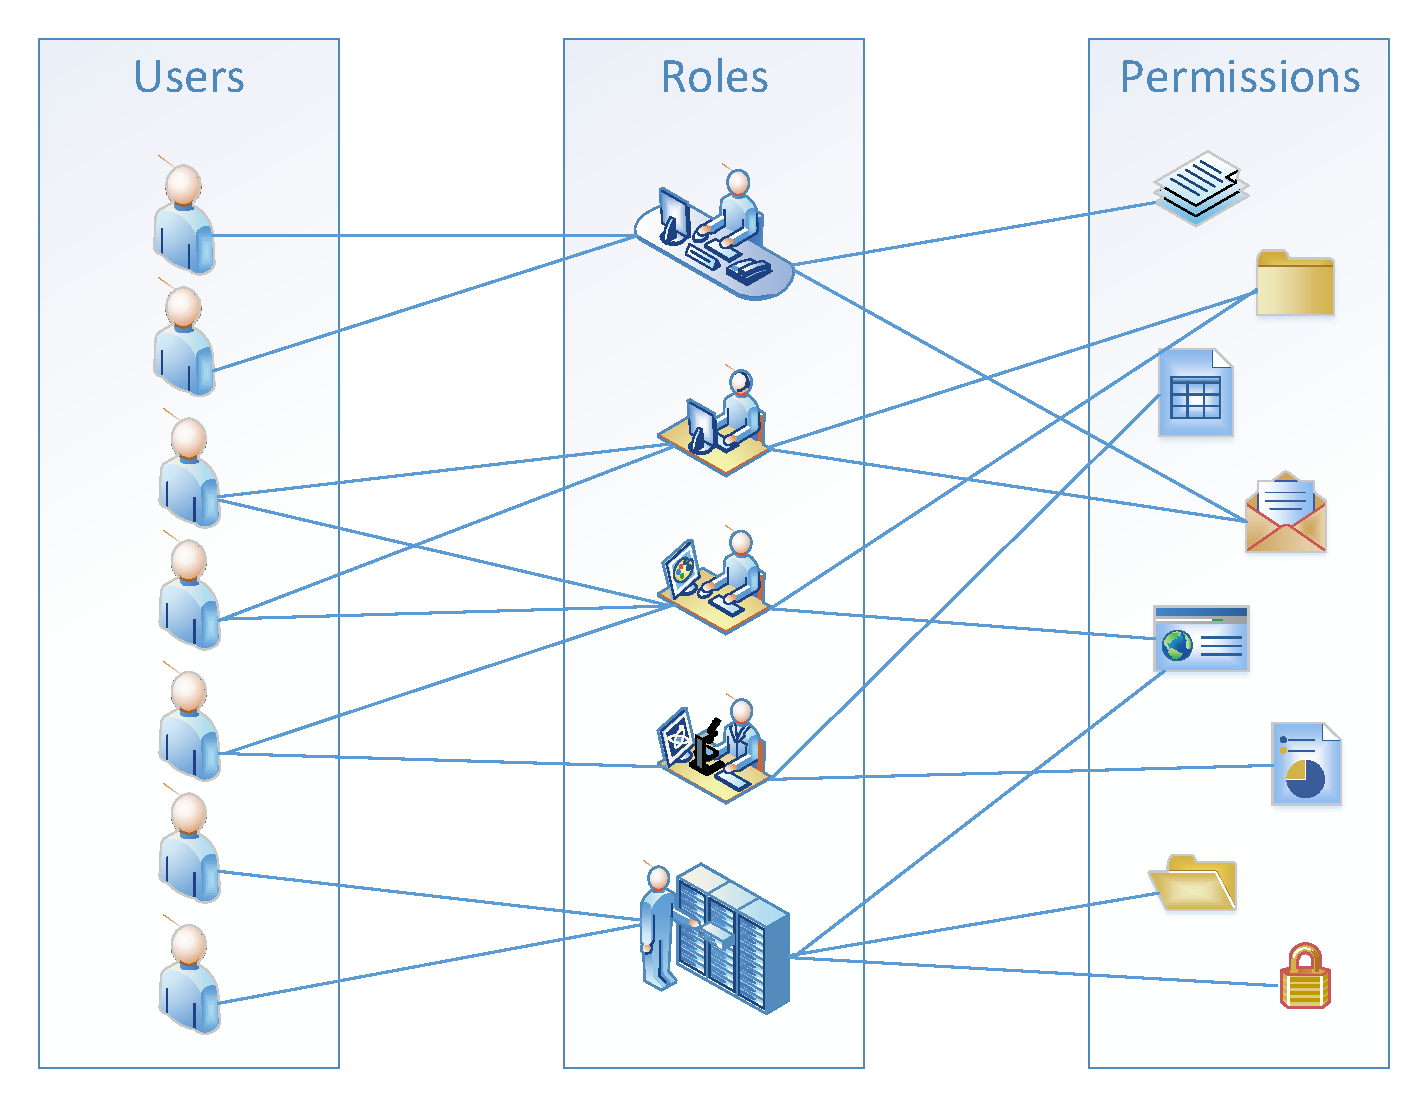
\includegraphics[scale=0.4]{User_Role_Perm}
                \caption{The relation between users, permission and roles in RBAC.}
                \label{fig:basicRBAC}
            \end{figure}
            
        \subsection{RBAC$_1$ - Role Hierarchies}
        \label{sec:rolehierarchies}
            The RBAC$_1$ model is based on RBAC$_0$ and introduces the concept of role hierarchies. In a role hierarchy roles can be assigned to roles and inherit their permissions to the roles they have been assigned to. The role hierarchy can be restricted as a tree or inverted tree, where a role inherits only the permissions of its child-roles, or a partially ordered set, where a role inherits the permissions from any other junior-role, which is assigned to it. It is also possible to limit inheritance in role hierarchies to control the power of impact of roles. In figure \ref{fig:rolehierarchies} shows one example of a role hierarchy.
            In Moffett\cite{Moffett:1998} role hierarchies and how they can be in conflict with some control principles, such as the Separation-of-Duty (SoD) principle, decentralisation, supervision and review, are discussed.
            \begin{figure}[H]
                \centering
                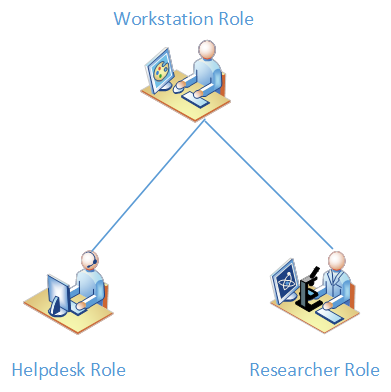
\includegraphics[scale=0.6]{Role_Hierarchy}
                \caption{Example of a role hierarchy: The Helpdesk Role and the Researcher Role are inheriting all the permissions from the Workstation Role and have some additional permissions.}
                \label{fig:rolehierarchies}
            \end{figure}
        \subsection{RBAC$_2$ - Constraints}
        \label{sec:rbac2}
            The RBAC$_2$ model is based on RBAC$_0$ and introduces the concept of constraints. With the help of constraints Separation-of-Duty (SoD), also known as Segregation-of-duty, can be achieved. SoD is a security principle for preventing fraud and errors by splitting tasks and associated permissions among multiple users. For example a user who has the permission to request the purchase of goods or services should not have the permission of approving the purchase. Roles in an RBAC model should therefore not have permissions bundled, which violate each other due to SoD. But also user assignments to multiple roles should not violate the SoD requirements.
        \subsection{RBAC$_3$ - Consolidated Model}
            The consolidated model combines RBAC$_1$ and RBAC$_2$ and therefore supports role hierarchies and constraints. Bringing these two functional capabilities together come with additional functionality. Constraints can also be applied on the role hierarchy. For example, the number of parent roles for child roles can be limited or different child roles can be constrained to have different parent roles.\\
    \begin{figure}[H]
        \centering
        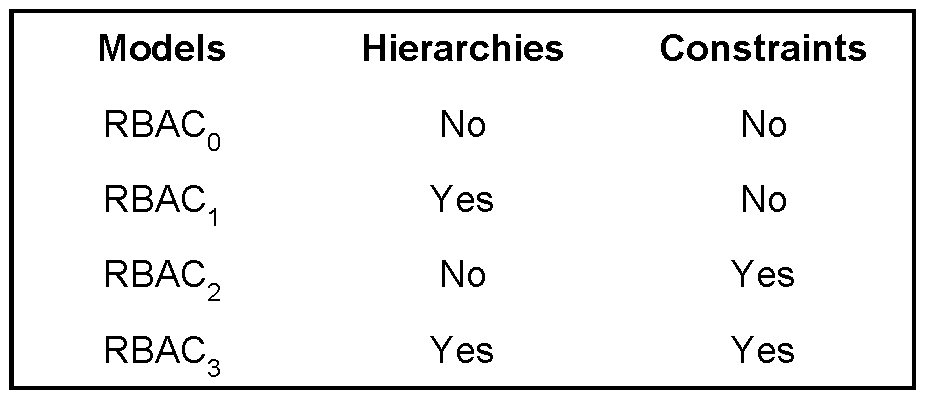
\includegraphics[scale=0.4]{RBAC_Models}
        \caption{(a) Relationship among RBAC models\cite{Sandhu:1996} (b) RBAC Definitions\cite{tassey2002economic}}
        \label{fig:rbacmodels}
    \end{figure}
    The relation of the four introduced models can be seen in figure \ref{fig:rbacmodels}. In this thesis the main focus will be on the RBAC$_0$ model. Like in Vaidya et al.\cite{Vaidya:2007} and Frank et al.\cite{Frank:2013} sessions will not be considered for simplicity reasons.\\
    The NIST RBAC model \cite{sandhu2000nist} distinguished between four levels of RBAC models: Flat, Hierarchical, Constrained and Symmetric RBAC. Each level introduces an additional functional capability to the previous level. In terms of the NIST RBAC model the Flat RBAC model will be the focus of the thesis.
    
    \section{Role Model Quality}
    \label{sec:rmQuality}
    A basic role model consists of users, permissions, roles, user-role assignments and role-permission assignments. A role model is most desirable if it has a state, which best leverages the RBAC model by satisfying the business, security and regulatory drivers: Lowering the costs for the administration of access control and equip employees with necessary permissions such that they can efficiently full-fill their tasks while keeping security requirements and being compliant.
    How this goal is measured in the role model has been described by several quality criteria\cite{Kunz}\cite{Frank}. The criteria concern the role model state, individual roles or both. In this thesis the different criteria is summarized into the categories: Completeness, complexity and comprehension.
        \subsection{Completeness}
        By completeness it is meant to rebuild the current user-permission assignment state by the role model. When the user-role and the permission-role assignments of the role model are resolved, it should cover all current user-permission assignments. In figure \ref{fig:roleminingExample} an example is shown where user-permission assignments are split into user-role and the permission-role assignments. Resolving an role model would be the other way around - from user-role and permission-role assignments to user-permission assignment.
        \iffalse
        \hl{(FEEDBACK:different scenarios: 1. starting from scratch, 2. already have assignments)}
        \fi
        \begin{figure}[H]
            \centering
            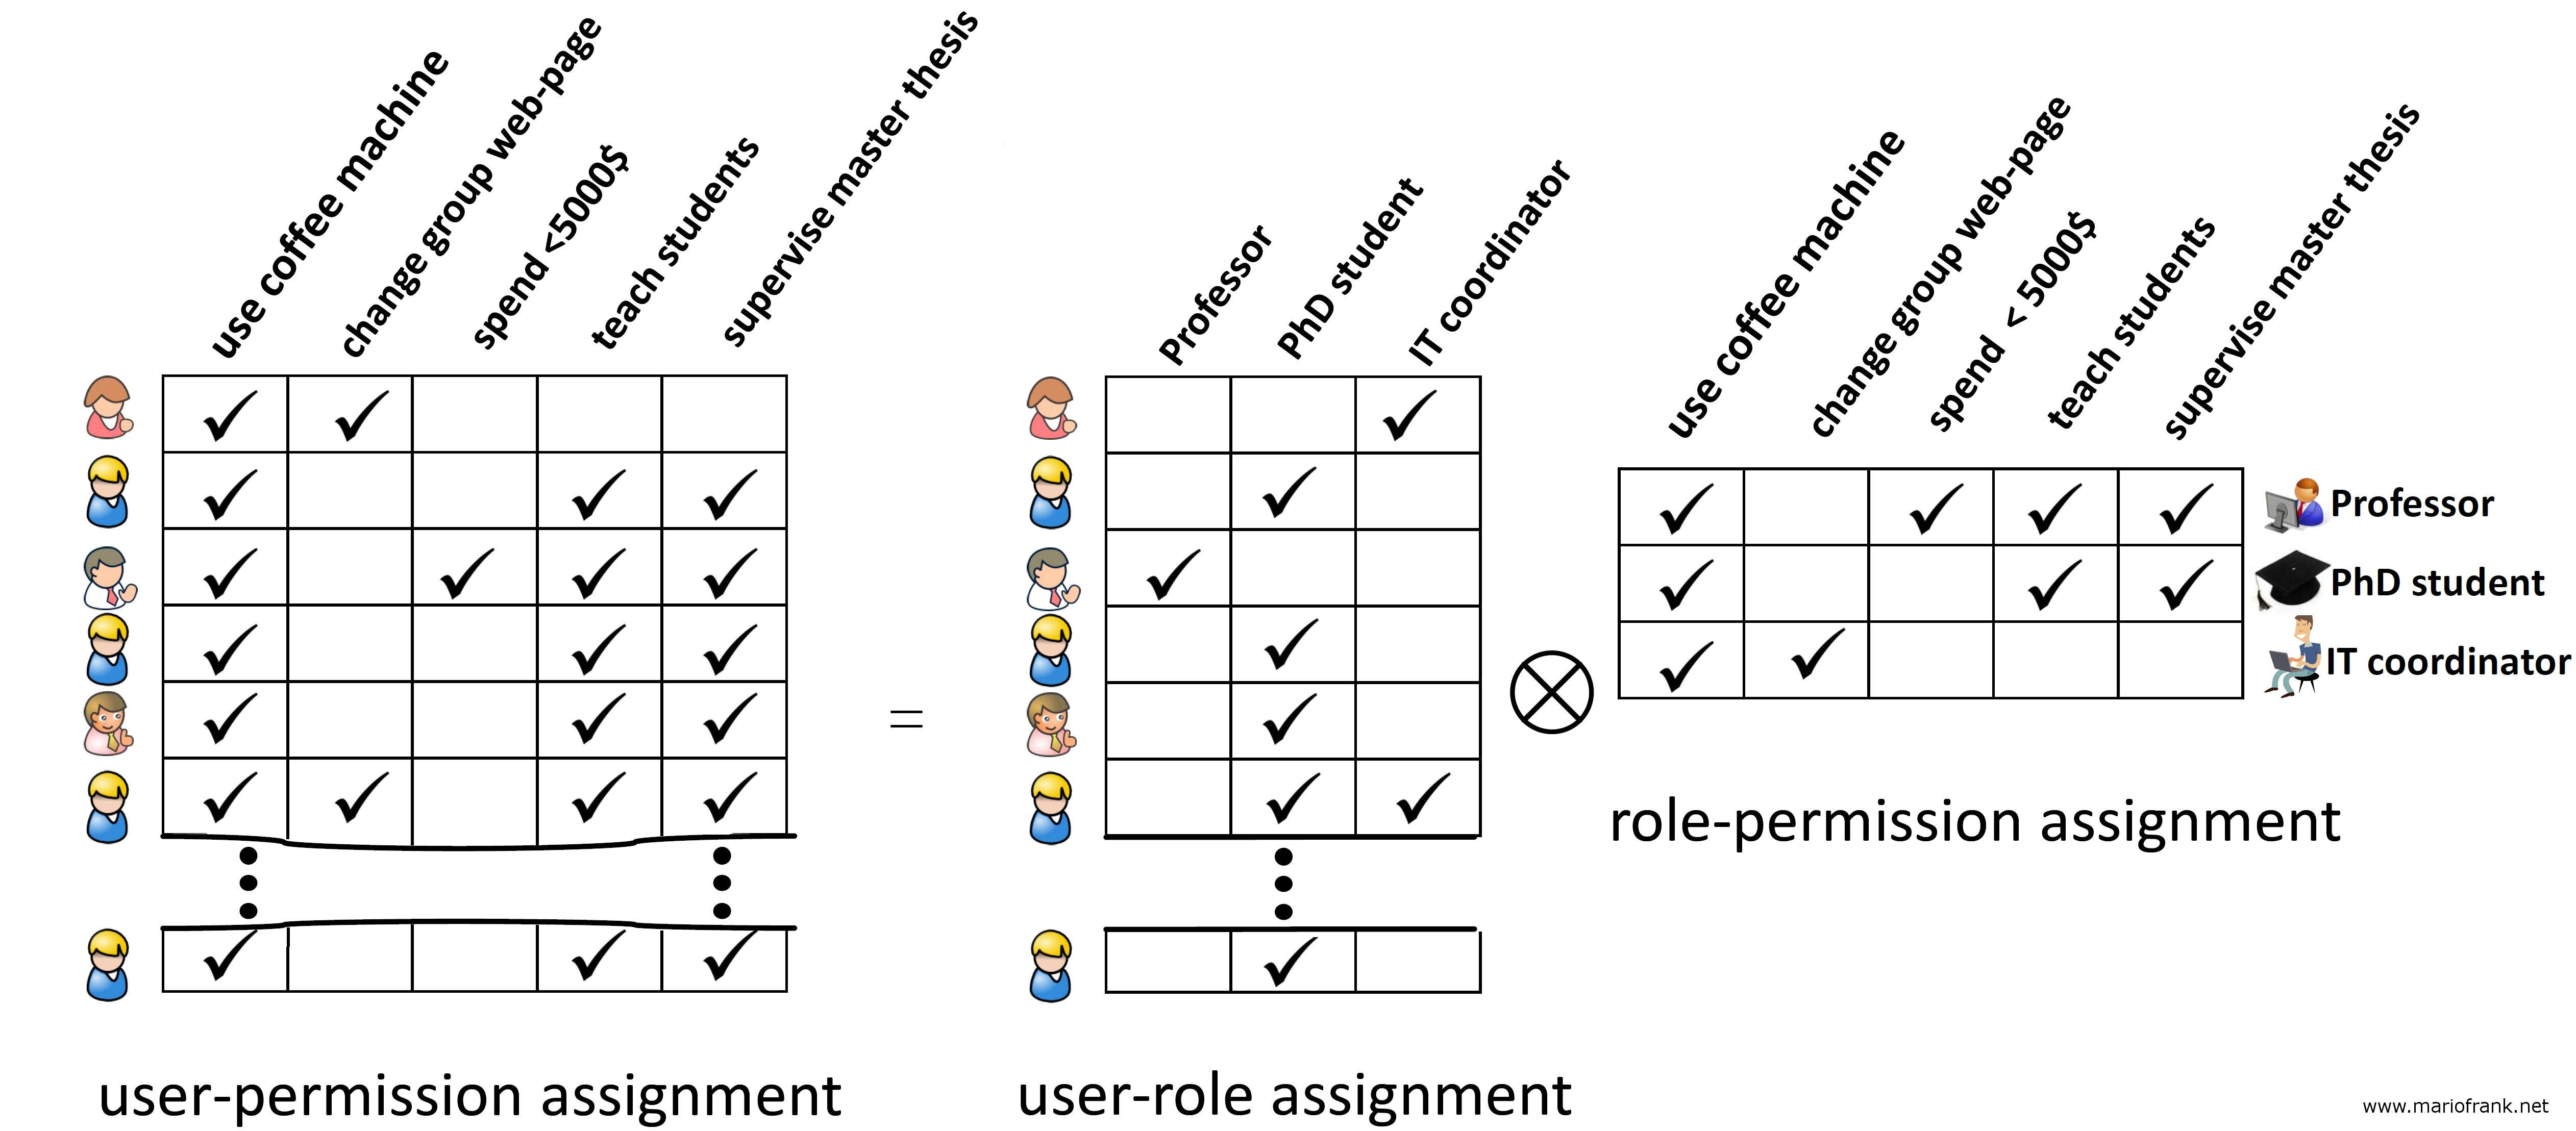
\includegraphics[scale=0.08]{RoleminingExample}
            \caption{University toy example taken from Frank\cite{roleMiningExample}, which demonstrates the transformation from user-permission assignment($UPA$) to user-role assignments($UA$) and permission-role assignments($PA$)}
            \label{fig:roleminingExample}
        \end{figure}
        It is assumed that the current user-permission assignments are in a state, where users get the necessary access to efficiently perform their tasks and no security or compliance regulations are violated. This of course is an ideal situation, but in reality the current state often has quite some noise, especially when no IAM solution has been in place before. Users tend to have more permissions than they actually need, since it is unlikely that someone will claim that he has too many permissions. The measure of completeness of the role model state is therefore in accordance to the initial access control configuration.\\
        A certain amount of overentitlements (users get too many permissions) or underentitlements (users get too few permissions) in the access control policies can be acceptable, if the least privilege principle is too costly to implement in practice. In figure \ref{fig:rolemodelComparison} an example of over- and underentitlements can be seen.
        \begin{figure}[H]
            \centering
            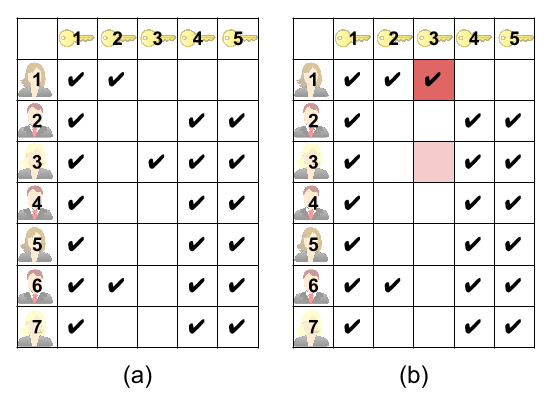
\includegraphics[scale=0.4]{RoleModel_Comparison}
            \caption{(a) Original user-permission assignments. There is a user for each row and a permission for each column. A check-mark represents the assigment of a permission to a user. (b) Resolved role model into user-permission assignments. In comparison to the original user-permission assignments one overentitlement (User 1 - Permission 3) and one underentitlement (User 3 - Permission 3) can be determined.}
            \label{fig:rolemodelComparison}
        \end{figure}
        The combinations of permissions within roles or the combination of user-role assignments might violate security regulations such as SoD. This measure is therefore not only taking individual roles but also the role model state into account.\\
        Constraints could also be ensured in a mechanism posterior to the role model, where individual permissions are detracted from users again, if it violates a constraint. Allowing constraint violations in the role model increases not only the processing and reliance on the posterior mechanism but also the auditing effort.
        \subsection{Complexity}
        The complexity of a role model is measured in its number of roles and the number of user-role and permission-role assignments. It is often connected to the maintenance costs of a role model. For example in figure \ref{fig:rolemodelComparison} three roles, eight user-role assignments and nine role-permission assignments can be counted.\\
        The more roles the role model has, the more maintenance effort is expected. Hence, a minimal set of roles is preferable. Furthermore it should be obvious that the total number of roles should be smaller than the total number of users or total number of permissions. Otherwise there would be no use of the advantage of having RBAC in comparison to IBAC in terms of administration costs. When each user has its individual role with the according individual bundle of permissions, the abstraction layer of the role becomes obsolete.\\
        Also the more user-role and permission-role assignments are needed, the more maintenance effort is expected. Large roles with many permissions may reduce the number of user-role assignments, but may lead to more confidentiality/accessibility violations (conflicting Completeness). The same applies for if each role is used by many users. Small roles with few permissions on the other hand can lead to more administration effort as mentioned above, since many roles are necessary for achieving completeness. The same applies if each role is only used by very few users.\\
        A role model can consists of very general large roles (e.g. a role for an organizational unit) and specialized small roles (e.g. a project-specific role). Determining a fix boundary of how many permissions or users can be assigned to a role requires knowledge of the role model or is given by company or security regulations.
        \subsection{Comprehension}
        A recently more discussed topic is the "meaningfulness" of roles \cite{Xu}\cite{Frank}. It is important that the administrators, which are maintaining the role model, can logically understand the role model for maintaining the roles and assignments confidently. Otherwise it might happen that they avoid to work with the role model since they feel not confident to stay in line with security and compliance regulations. Or it will cause them extra effort and costs to work with the role model. The roles should be therefore comprehensive, which can be achieved by giving them a meaning close to business roles, e.g. a role "Employee", which contains all permissions every employee will get and is assigned to every employee-user.\\
        This criteria can loosen some of the other criteria, which rather concentrate on the compression of the access control information \cite{Frank:2013}. For achieving more intuitive meaningful roles it might be necessary to allow more roles than the minimal number of roles resulting from compression. More roles might result in more assignments, which are necessary to keep the role model more comprehensive. Lowering costs by having a more comprehensive role model may contradict lowering costs by having a less complex role model.
        \iffalse
        In praxis the roles can be often bundled according to the user attributes Internal or External employee, Organizational Unit and Job Function. The pyramid in figure \ref{fig:rolePyramid} demonstrates how easily user-permission assignments can be covered by roles.
        \begin{figure}[H]
            \centering
            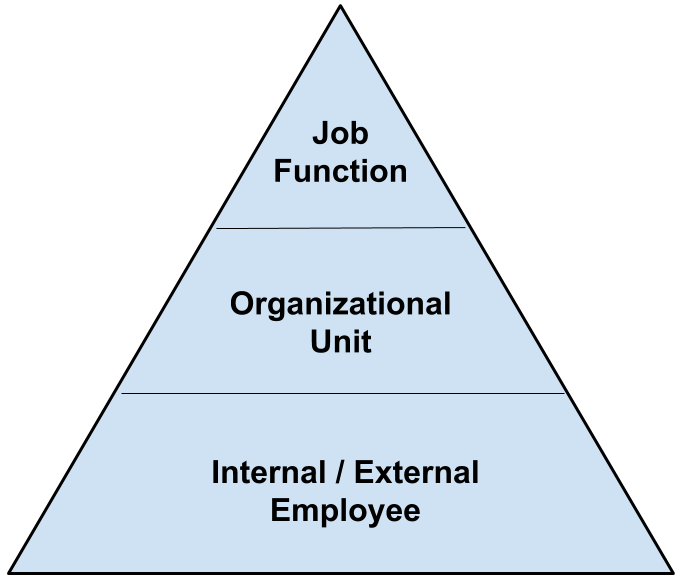
\includegraphics[scale=0.3]{Role_Pyramid}
            \caption{Pyramid of general roles depending on user attributes. Most often roles can be described by the user attributes Internal or External employee, Organizational Unit and Job Function.}
            \label{fig:rolePyramid}
        \end{figure}
        \fi
    
    \section{Role Engineering}
    Role engineering \cite{Coyne:2011} describes the process to create a role model for RBAC. This task is proved to be very difficult in large enterprises.\\
    There are three different approaches to conquer the goal of finding the right role model: Top-Down, Bottom-Up and the Hybrid approach\cite{Coyne:2011}\cite{Frank}.
    \begin{itemize}
        \item \textbf{Top-Down Approach}\\
        One approach is to do a top-down analysis, where the roles are built out of business information. Business processes, business roles and security policies are analysed to build a suitable role model. The resulting roles contain high-level permissions, which need to be mapped to technical permissions that are used by IT systems. The roles are easy to understand as they are derived from business concepts. The analysis of the business information by experts to a high-level role model and the mapping into low-level accesses by IT Specialists are very time-consuming and costly. Furthermore the resulting role model could lead to a different access control configuration than the current one. It is likely that users get less permissions than they used to have, which might prevent them of doing their tasks efficiently.
        \item \textbf{Bottom-Up Approach}\\
        The bottom-up approach exploits the current user-permission assignments and tries to gather a role model out of it. Since this approach often uses Data Mining Techniques, the method is also called Role Mining\cite{Kuhlmann}. This approach on the other hand is often failing in generating a comprehensive role model, which is accepted by the administrators\cite{Frank:2013}.
        \item \textbf{Hybrid approach}\\
        Since the advantages and disadvantages of the top-down and the bottom-up approach are mirrored, hybrid approaches have been suggested \cite{Frank}\cite{6274146}. In these approaches the business information is leveraged to guide the computational generation of a role model out of user-permission assignments.
    \end{itemize}
    A role model is evolving over time and needs constant maintenance\cite{Montrieux:2011}. Administrators and Re-attestation processes are changing the user-permission assignments by adding and removing users and permissions to and from roles. New users are joining and others get removed, same is valid for applications and their permissions. Separate access control configurations might need to be migrated to one access control configuration. The task of role engineering is therefore not a one time task, but an on-going process. An over-the-time suboptimal role model can increase the administration costs and has to be optimized again to benefit from the advantages of RBAC.
    
    \section{Role Mining}
    Role Mining is a bottom-up role engineering approach. The basic input of role mining are users, permissions and the current assignments to each other. The input can be expressed as tuple $<U,P,UPA>$, where
    \begin{itemize}[noitemsep,topsep=0pt,parsep=0pt,partopsep=0pt]
        \item \textbf{$U$} is a set of users
        \item \textbf{$P$} is a set of permissions
        \item \textbf{$UPA \subseteq U \times P$} are user-permission assignments
    \end{itemize}
    On top additional information can be taken as input like constraints, top-down information (business information) and already existing roles. The output of role mining is the role model. A basic role model state can be described as tuple $<U,P,R,UA,PA>$, where
    \begin{itemize}[noitemsep,topsep=0pt,parsep=0pt,partopsep=0pt]
        \item \textbf{$U$} is a set of users
        \item \textbf{$P$} is a set of permissions
        \item \textbf{$R$} is a set of roles
        \item \textbf{$UA \subseteq U \times R$} are user-role assignments
        \item \textbf{$PA \subseteq R \times P$} are permission-role assignments
    \end{itemize}
    Optionally a role hierarchy is also part of the role model. In some papers, such as \cite{Molloy} and \cite{DuChang}, direct user-role assignments ($DUPA \subseteq U \times P$) are added to the role model tuple in order to provide more flexibility to handle anomalous permissions which do not fit into the role structure. Alternatively a new role for each of the individual direct assignments of DUPA can be defined, although such roles are not desirable in a role model. By adding DUPA to the tuple it can be distinguished between DUPA and undiserable roles. Figure \ref{fig:rolemining} shows the inputs and outputs of the role mining process.  A specific example in matrix representation is shown in figure \ref{fig:roleminingExample}.
    \begin{figure}[H]
        \centering
        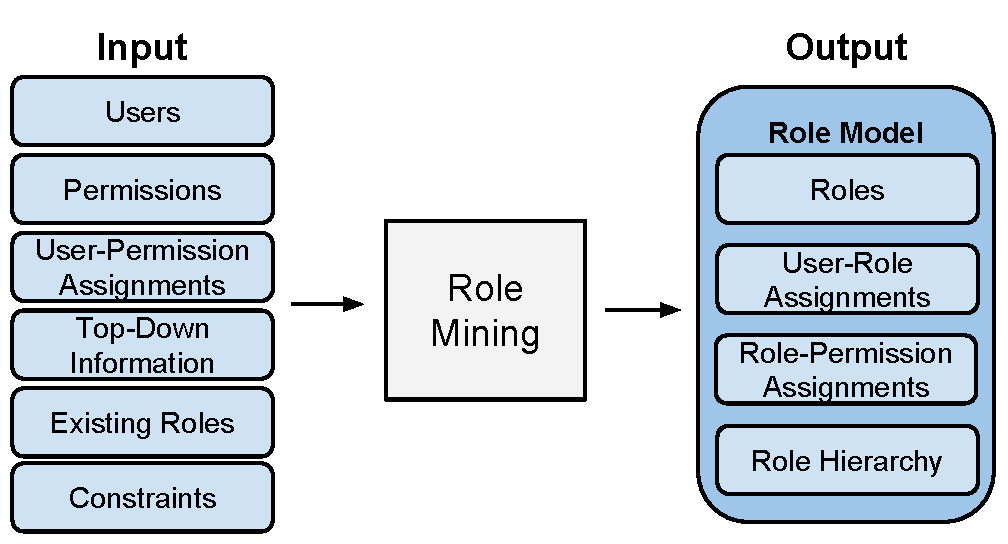
\includegraphics[scale=0.4]{Rolemining}
        \caption{The inputs and outputs of the role mining process}
        \label{fig:rolemining}
    \end{figure}
    
    \subsection{Role Mining Problem Definitions}
    \label{sec:roleMiningProblems}
    There are several role-mining problem (RMP) definitions existing. The problem definitions, which will be referred to in this thesis, are introduced in the following.
    \begin{itemize}
        \item \textbf{The Basic Role-Mining Problem}\cite{Vaidya:2007}\\
        \textit{"Given a set of users $U$, a set of permissions $P$ and a user-permission assignment $UPA$, find an RBAC configuration $RC$ that minimizes the number of roles $k$ and does not deviate from $UPA$."}
        \item \textbf{The $\delta$-approx. Role-Mining Problem}\cite{Vaidya:2007}\\
        \textit{"Given a set of users $U$, a set of permissions $P$ and a user-permission assignment $UPA$, find an RBAC configuration $RC$ that minimizes the number of roles $k$ and deviates from $UPA$ with less than $\delta$ assignments."}
        \item \textbf{The Min-Noise Role-Mining Problem}\cite{Vaidya:2007}\\
        \textit{"Given a set of users $U$, a set of permissions $P$ and a user-permission assignment $UPA$, and the number of roles $k$, find an RBAC configuration $RC$ with $k$ roles, minimizing the deviation between $UPA$ and $RC$."}
        \item \textbf{The Min-Edge Role-Mining Problem}\cite{4497438}\\
        \textit{"Given a set of users $U$, a set of permissions $P$ and a user-permission assignment $UPA$, find an RBAC configuration $RC$ that is consistent with $UPA$ and minimizes the number user-role assignments and role-permission assignments."}
        \item \textbf{The Interference Role-Mining Problem}\cite{Frank:2013}\\
        \textit{"Let a set of users $U$, a set of permissions $P$, a user-permission relation $UPA$, and, optionally, part of the top-down information $TDI$ be given. Under Assumption 1-3, infer the unknown RBAC configuration $RC*=(R*, UA*, PA*)$.\\
        Assumptions:\\
        1. $RC*$ generated $UPA$\\
        2. $RC*$ reflects top-down information ($TDI$).\\
        3. Exceptions (errors) might exist."}
    \end{itemize}
    \subsection{Related Problem: Boolean Matrix Decomposition Problem}
    The role mining problem is related to the Boolean Matrix Decomposition (BMD) Problem. In Lu et al.\cite{4497438} the RMP is first modelled as BMD, where a binary matrix is decomposed into two matrices. The combination of these matrices results into the original matrix. Several different decompositions can exist for a matrix.
    \begin{itemize}
    \item \textbf{Boolean Matrix Multiplication Definition:}\\
    $C = A \times B$ is the boolean matrix multiplication between boolean matrices $A \in \{0,1\}^{m \times k}$ and $B \in \{0,1\}^{k \times n}$. The product $C$ is a boolean matrix with $m \times n$ dimension and is calculated with $c_{ij} = \bigvee_{l=1}^{k}(a_{ij} \wedge b_{ij})$
     \item \textbf{Boolean Matrix Decomposition Problem Definition:}\\
    The BMD problem is an optimization problem where given a boolean matrix $C \in \{0,1\}^{m \times n}$, the boolean matrices $A \in \{0,1\}^{m \times k}$ and $B \in \{0,1\}^{k \times n}$ have to be found, such that $C = A \times B$ and $k$ is minimal\cite{vaidya2012boolean}. $A \times B$ is called a decomposition of $C$.
    \end{itemize}
    For RMP a user-permission assignment matrix ($C$) needs to be decomposed into a user-role assignments matrix ($A$) and a role-permission assignments matrix ($B$). Variable $k$ then represents the number of roles, variable $m$ and $n$ the number of users and permissions accordingly. Therefore finding the minimal $k$ in the BMD problem corresponds to finding the minimal number of roles in the basic RMP. The notion of BMD for the RMP is also used in this thesis and has been already introduced in previous sections (see Figure \ref{fig:roleminingExample} and \ref{fig:rolemodelComparison}).
\newline
\newline
In this thesis the role mining problem is tackled with evolutionary algorithms. An introduction to evolutionary algorithms is given in the next chapter.